%! TeX program = lualatex
\documentclass[10pt,a4paper,table]{article}

\usepackage{amsmath,amssymb,amsthm,mathtools,amsfonts}
\usepackage{breqn}
\usepackage[utf8]{inputenc}
\usepackage[danish]{babel}
\usepackage[T1]{fontenc}

%%%%%%%%%%%%%%%%%%%%%%%%%%%%%%%%%%%%%%%%%%%%%%%%%%%%%%%%%%%%%%%%%%%%%%%%%%%%%% Fonts

\usepackage{fontspec}
\setmainfont{Times New Roman}
\newfontfamily\garamond[Numbers=OldStyle]{EB Garamond}
\newfontfamily\plantin[Numbers=OldStyle]{Plantin MT Pro}
\newfontfamily\wal{Walbaum Com}
\newfontfamily\klav{Klavika}
\newfontfamily\klavl{Klavika light}
\newfontfamily\quotefont[Ligatures=TeX]{Linux Libertine O}
\newfontfamily\vest{TRY Vesterbro Regular}
\newfontfamily\vestb{TRY Vesterbro Poster}
\newfontfamily\overp{Overpass}

%%%%%%%%%%%%%%%%%%%%%%%%%%%%%%%%%%%%%%%%%%%%%%%%%%%%%%%%%%%%%%%%%%%%%%%%%%%%%% Colors

\usepackage{xcolor}
\usepackage{transparent}

\definecolor{frbblue}{RGB}{47, 88, 109}
\definecolor{hgred}{RGB}{140, 10, 10}
\definecolor{frbgreenl}{RGB}{162, 202, 137}
\definecolor{frbgreen}{RGB}{28, 85, 66}
\definecolor{frbgrey}{RGB}{243, 245, 242}

%%%%%%%%%%%%%%%%%%%%%%%%%%%%%%%%%%%%%%%%%%%%%%%%%%%%%%%%%%%%%%%%%%%%%%%%%%%%%% Other Graphics

\usepackage{graphicx}
\graphicspath{{../img/}}
\usepackage{tikz}
\usetikzlibrary{calc}
\usepackage{placeins}

\usepackage[pdfborder={0 0 0}]{hyperref}

\usepackage{multicol}
\usepackage{cellspace}
\setlength\cellspacetoplimit{100pt}
\setlength\cellspacebottomlimit{100pt}
\usepackage{tabularx}
\newcolumntype{b}{>{\hsize=\hsize}>{\centering\arraybackslash}X}
\usepackage{siunitx}
\setlength\cellspacetoplimit{4pt}
\setlength\cellspacebottomlimit{4pt}

\usepackage{enumitem}
\usepackage{wrapfig}
\usepackage{caption}
\usepackage{titlesec}

\setlength{\parskip}{0.5\baselineskip}
\setlength{\parindent}{0cm}
\setlist[enumerate]{label=\alph*),left=20pt}

%%%%%%%%%%%%%%%%%%%%%%%%%%%%%%%%%%%%%%%%%%%%%%%%%%%%%%%%%%%%%%%%%%%%%%%%%%%%%% New commands

\newcommand\svar[1]{\newline\textcolor{red}{\textbf{Svar}\\#1}}

\usepackage[h]{esvect}
\newcommand{\twvect}[2]{\ensuremath{\begin{pmatrix}#1\\#2\end{pmatrix}}}

\newcommand*\quotesize{20}
\newcommand*{\openquote}
  {\tikz[remember picture,overlay,xshift=-3ex,yshift=-0ex]
    \node (OQ) {\quotefont\fontsize{\quotesize}{\quotesize}\selectfont``};\kern0pt}

\newcommand*{\closequote}[1]
  {\tikz[remember picture,overlay,xshift=2ex,yshift={#1}]
    \node (CQ) {\quotefont\fontsize{\quotesize}{\quotesize}\selectfont''};}

\newcommand{\qm}[1]{``#1''}
\newcommand{\iquote}[1]{\begin{quote}\itshape \openquote#1\hfill\closequote{0ex} \end{quote}}

%%%%%%%%%%%%%%%%%%%%%%%%%%%%%%%%%%%%%%%%%%%%%%%%%%%%%%%%%%%%%%%%%%%%%%%%%%%%%% Sections
\usepackage{chngcntr}

\renewcommand\thesection{\arabic{section}}

\titleformat{\section}[block]
  {\flushright\overp\Large\color{frbgreen}}
  {}
  {0pt}
  {\clearpage EKSTRA}
  [{\color{frbgreenl}\vspace{-1em}\hspace*{-0.165\linewidth}\rule{\dimexpr1.165\linewidth\relax}{0.4pt}\kern1mm}]

\counterwithout{subsection}{section}
\renewcommand\thesubsection{Opgave \arabic{subsection}}
\titleformat{\subsection}[leftmargin]{\bfseries}{}{0pt}{\hspace{-5em}\thesubsection}

%%%%%%%%%%%%%%%%%%%%%%%%%%%%%%%%%%%%%%%%%%%%%%%%%%%%%%%%%%%%%%%%%%%%%%%%%%%%%% Header & Footer

\usepackage{bigfoot}
\DeclareNewFootnote{a}
\renewcommand{\thefootnotea}{\fnsymbol{footnotea}}
\newcommand{\footnotes}[1]{\footnotea[2]{#1}}
\MakePerPage{footnotes}

\usepackage{fancyhdr}
\fancypagestyle{plain}{%
  \setlength{\headheight}{60pt}%
  \setlength{\headsep}{0pt}
  \fancyhf{}
  \renewcommand{\footrulewidth}{0pt}%
  \renewcommand\headrule{}%
  \fancyhead[L]{}
  \fancyhead[C]{}
  \fancyhead[R]{\overp\color{frbgreenl}\normalsize \overp Mat C-B\\\huge\color{frbgreen}\vestb Geometri repetition}
  \cfoot{\thepage}
}
\pagestyle{fancy}
\fancyhf{}
\renewcommand\headrule{}
\lhead{}
\rhead{}
\cfoot{\thepage}

%%%%%%%%%%%%%%%%%%%%%%%%%%%%%%%%%%%%%%%%%%%%%%%%%%%%%%%%%%%%%%%%%%%%%%%%%%%%%% Document

\begin{document}
\thispagestyle{plain}
\begin{tikzpicture}[remember picture,overlay]
    \node[anchor=north west,yshift=-48pt,xshift=120pt,opacity=0.2]%
        at (current page.north west)
        {
\includegraphics[scale=0.25]{frbvuc_logo.png}};
\end{tikzpicture}
\begin{tikzpicture}[remember picture,overlay]
  \definecolor{bgline}{RGB}{205,214,208}
  \coordinate (C) at ($(current page.north)+(35mm,-5mm)$);
  \draw[bgline, line width=0.6pt] (C) circle (65mm);
  \draw[bgline, line width=0.4pt]
    ($(current page.north east)+(0,0mm)$) ++(-28mm,0)
    -- ($(current page.south east)+(0,10mm)$) ++(-28mm,0);
\end{tikzpicture}


\subsection{}

Bestem afstanden $|AB|$ mellem punkterne $A(2, 1)$ og $B(14, 6)$.


\subsection{}

To linjer er givet ved
\[
  l: y = 1{,}5x - 8 \qquad \text{og} \qquad m: y = -0{,}5x + 16
\]
Bestem koordinaterne til skæringspunktet $S$ mellem $l$ og $m$.


\subsection{}

En linje er givet ved $l: y = 3x - 2$.

Bestem linjens hældningsvinkel $v$.


\subsection{}

Bestem afstanden $d$ fra punktet $P(2, 4)$ til linjen $l: y = 3x + 7$.


\subsection{}

En cirkel har centrum $C$ på $x$-aksen. Tangenten til cirklen i punktet $P(0, 4)$ er linjen $l: y = 2x + 4$.

\begin{enumerate}
  \item Bestem koordinaterne til centrum $C$.
  \item Bestem cirklens ligning.
\end{enumerate}


\subsection{}

En cirkel $k$ er givet ved $(x-5)^2 + (y+1)^2 = 13$.

Bestem ligningerne for de to tangentlinjer $t_1$ og $t_2$ til $k$, der er parallelle med $y$-aksen.


\subsection{}

En cirkel er givet ved $(x-6)^2 + (y-3)^2 = 25$ og en linje er givet ved $l: y = 0{,}75x + 8$.

\begin{enumerate}
  \item Bestem afstanden fra cirklens centrum til linjen $l$.
  \item Afgør, om $l$ skærer, tangerer eller ikke rammer cirklen.
\end{enumerate}


\subsection{}

To parabler er givet ved
\[
  f(x) = 0{,}5x^2 - x + 3 \qquad \text{og} \qquad g(x) = -0{,}5x^2 + 2x + 3
\]

\begin{enumerate}
  \item Bestem koordinaterne til skæringspunkterne $P$ og $Q$ mellem de to parabler.
  \item Bestem vinklen som linjen $PQ$ danner med $y$-aksen.
\end{enumerate}


\subsection{}

To cirkler er givet ved
\[
  C_1{:}\ (x-54)^2 + (y-34)^2 = 515{,}29 \qquad \text{og} \qquad C_2{:}\ \text{centrum } (109, 106),\ r_2 = 5
\]
Bestem den mindste afstand mellem de to cirklernes rande.


\subsection{}

Funktionen $f$ er givet ved $f(x) = 0{,}5 + 4x - 2{,}5^x$. Punktet $P(1, 2)$ ligger på grafen for $f$.

\begin{enumerate}
  \item Bestem ligningen for tangenten $t$ til grafen for $f$ i punktet $P$.
  \item Bestem ligningen for den vinkelrette linje $l$ til $t$ i punktet $P$.
\end{enumerate}


\subsection{}

En cirkel har ligningen $(x-1)^2 + (y-4)^2 = 9$.

\begin{enumerate}
  \item Bestem centrum og radius for cirklen.
  \item Undersøg, om punktet $P(5, 6)$ ligger på cirklen.
\end{enumerate}


\subsection{}

To linjer er givet ved
\[
  l: y = ax + 6 \qquad \text{og} \qquad m: y = 5x - 2
\]
Det oplyses, at linjerne $l$ og $m$ er ortogonale (vinkelrette på hinanden).

Bestem tallet $a$.


\subsection{}

En linje $l$ er givet ved ligningen $0{,}75x - y + 2 = 0$, og et punkt er givet ved $P(7, 1)$.

\begin{enumerate}
  \item Bestem afstanden fra punktet $P$ til linjen $l$.
  \item Linjen $l$ er tangent til en cirkel $C$ med centrum i punktet $P$. Bestem en ligning for cirklen $C$.
  \item En linje $m$ står vinkelret på $l$. Bestem hældningskoefficienten for $m$.
\end{enumerate}


\subsection{}

I et koordinatsystem er der givet et punkt $P(1, 3)$ og en linje $l$ med ligningen $y = 0{,}75x + 1$.

\begin{enumerate}
  \item Bestem afstanden fra punktet $P$ til linjen $l$.
  \item Cirklen $C$ har centrum i punktet $P$ og linjen $l$ som tangent. Bestem en ligning for cirklen $C$.
\end{enumerate}


\subsection{}

En ret linje er givet ved ligningen $y = 5x - 21$, og en cirkel er givet ved $(x-2)^2 + (y-10)^2 = 17$.

\begin{enumerate}
  \item Bestem hældningsvinklen for linjen.
  \item Bestem centrum og radius for cirklen.
  \item Bestem afstanden fra cirklens centrum til linjen, og brug resultatet til at afgøre, om linjen er tangent til cirklen.
\end{enumerate}


\subsection{}

I et koordinatsystem er der givet et punkt $P(4, 1)$ og en linje $l$ med ligningen $y = 0{,}25x + 2$.

\begin{enumerate}
  \item Bestem afstanden fra punktet $P$ til linjen $l$.
  \item Linjen $m$ går gennem $P$ og står vinkelret på $l$. Bestem en ligning for linjen $m$.
  \item Bestem hældningsvinklen for linjen $m$.
\end{enumerate}


\subsection{}

To cirkler er givet ved
\[
  k_1{:}\ (x-2)^2 + (y-3)^2 = 16 \qquad \text{og} \qquad k_2{:}\ \text{centrum } (7, 15),\ r_2 = 3
\]

\begin{enumerate}
  \item Bestem centrum og radius for cirklen $k_1$.
  \item Bestem den mindste afstand mellem de to cirklernes rande.
\end{enumerate}


\subsection{}

En cirkel er givet ved $x^2 + (y-6)^2 = 8$, og røringspunktet $P(2, 4)$ ligger på cirklen.

\begin{enumerate}
  \item Bestem en ligning for tangenten $t$ til cirklen i punktet $P$.
  \item En større cirkel har centrum i $C(13, 6)$, og tangenten $t$ er også tangent til den større cirkel. Bestem radius for den større cirkel.
\end{enumerate}


\subsection{}
\
\begin{figure}[h!]
\centering
\vspace{-15pt}
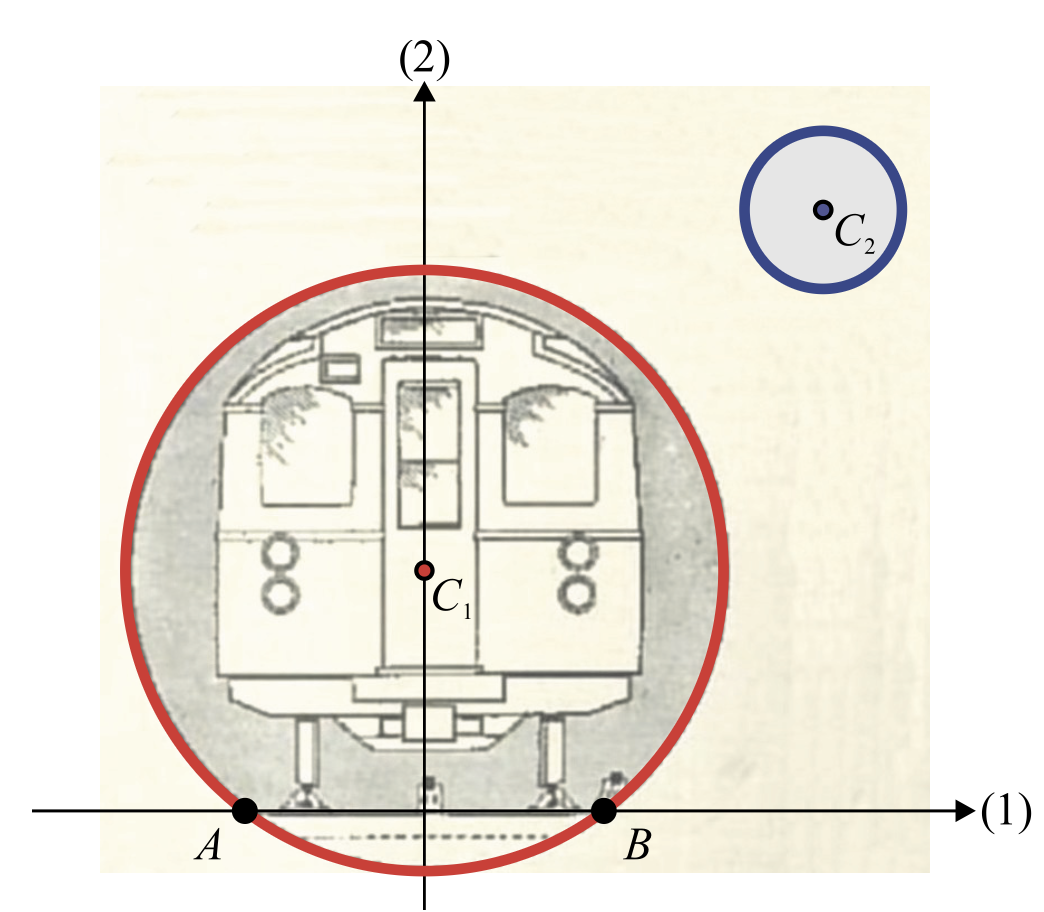
\includegraphics[width=0.50\textwidth]{tunnel}
\end{figure}

Figuren viser et tværsnit af en tunnelbane indlagt i et koordinatsystem, hvor bunden af tunnelen ligger på førsteaksen. Alle mål er i meter. Den røde cirkel på figuren har centrum i $C_1(0,\ 1{,}2)$ og radius $r_1 = 1{,}5$.

\begin{enumerate}
  \item Bestem en ligning for den røde cirkel.
\end{enumerate}

Linjestykket $AB$ udgør bunden af tunnelen, se figuren.

\begin{enumerate}[resume]
  \item Bestem længden af $AB$.
\end{enumerate}

Den blå cirkel på figuren viser et tværsnit af et kloakrør. Den blå cirkel har centrum i $C_2(2,\ 3)$ og radius $r_2$.

Den mindste distance mellem den røde cirkel og den blå cirkel er $0{,}8$ meter.

\begin{enumerate}[resume]
  \item Bestem radius $r_2$ i den blå cirkel.
\end{enumerate}


\subsection{}

I et koordinatsystem har en cirkel ligningen $(x-3)^2 + (y-2)^2 = 25$.

\begin{enumerate}
  \item Bestem radius og koordinaterne til centrum.
  \item Linjestykket $AB$ er en diameter i cirklen, og punktet $A$ ligger på $y$-aksen. Bestem koordinaterne til $A$ og $B$ i begge mulige tilfælde.
  \item Bestem den spidse vinkel mellem de to diametre.
\end{enumerate}


\end{document}

%%%%%%%%%%%%%%%%%%%%%%%%%%%%%%%%%%%%%%%%%%%%%%%%%%%%%%%%%%%%%%%%%%%%%%%%%%%%%% Skabeloner

% Sidestillet figur
\begin{wrapfigure}[8]{r}{0.2\textwidth}
\vspace{-18pt}
\includegraphics[width=0.3\textwidth]{ovn}
\end{wrapfigure}

% Midterstillet figur
\begin{figure}[h!]
\centering
\includegraphics[width=0.8\textwidth]{abc}
\end{figure}

% Førstillet figur
\
\begin{figure}[h!]
\centering
\vspace{-15pt}
\includegraphics[width=0.35\textwidth]{stud}
\end{figure}

% Tabel
\begin{figure}[h!]
\centering\renewcommand{\arraystretch}{1.5}
\begin{tabularx}{0.9\textwidth}{|l|b|b|b|b|b|b|}
	\hline \cellcolor{hggreen} Decimaltal & 7\% & -51\% & 13,7\% & 126\% & 456\% & 0,28\%\\\hline
	\cellcolor{hggreen} Procenttal &  &  &  &  &  & \\\hline
\end{tabularx}
\end{figure}

% Forklaringsopgaver
\begin{align*}
&&	&						&&\underset{\rule{0.8\linewidth}{0pt}}{\textbf{Forklaring:}}\\[1em]
&&	&\frac{(x+2)^2 - 4}{x} 		&&\underset{\rule{0.8\linewidth}{0.4pt}}{\text{Udtrykket skrives op.}}\\[2em]
&&	=&\ \frac{x^2 + 4 + 4x - 4}{x}	&&\underset{\rule{0.8\linewidth}{0.4pt}}{\text{}}\\[2em]
&&	=&\ \frac{x^2 + 4x}{x}			&&\underset{\rule{0.8\linewidth}{0.4pt}}{\text{}}\\[2em]
&&	=&\ x + 4					&&\underset{\rule{0.8\linewidth}{0.4pt}}{\text{}}\\[2em]
\end{align*}

% Sørg for at figur er placeret før et vidst sted
\FloatBarrier
